% !TeX root = ../../thesis.tex
\chapter{Conclusion}\label{ch:conclusion}


Each chapter of this thesis consists of an independent scientific study and includes its own detailed discussion. Consequently, this chapter provides a general summary and conclusion of the current PhD research. Moreover, it includes an overview of the limitation and challenges we needed to tackle during the project, as well as suggested future directions and contributions to continue this piece of work.

\section{Project summary}

% overview of chapters and objectives

This PhD thesis presented a mechanistic model of the biodegradation process of metallic biomaterials, with a focus on the \textit{in vitro} Mg biodegradation. For achieving this goal, the project was divided into several work packages, each of which containing a specific goal to reach, as described in Chapter \ref{ch:objective}. The research carried on in this PhD thesis lies where biomedical engineering, materials science, mathematics, and computational sciences collide. The relevant elements of these disciplines were employed in a multidisciplinary manner to deliver a multiphysics model of the chemistry of biodegradation by considering the effect of the environment determined by the final application. After developing the model, it has been used in multiple case-studies to demonstrate the integration capabilities, which was one of the initial goals of the project.

As stated in Chapter \ref{ch:introduction}, building a mechanistic model of the biomaterials biodegradation for any arbitrary shape in 3D can be challenging. Despite the technical challenges, such a model can provide more accurate predictions of the underlying processes in comparison to data-driven and stochastic models. In order to build the core computational model, the chemical reactions occurring at the interface of Mg during the biodegradation were converted to corresponding mathematical forms, a set of reaction-diffusion PDEs. Since studying the change of the morphology of the implants and medical devices can be beneficial for the design optimization processes, it was essential for the model to be able to capture the morphological changes in the shape of the simulated 3D objects. For doing this, an interface tracking technique, formulated using the level-set method, was integrated into the biodegradation model, enabling us to capture the movement of the corrosion front due to loss of materials. This model was capable of reproducing the basic biodegradation behavior of commercially-pure Mg in saline and buffered solutions, typical test environments to evaluate the corrosion behavior of metallic materials. 

Due to the complexity of the derived mathematical model, it was more convenient to implement it in an in-house code with full control on the details of numerical solution and computational implementation. More elaboration on this choice will be discussed in Section \ref{sec:open_source}. The resulting coupled equations were solved using the finite element method implemented in the open-source domain-specific language FreeFEM, in which a wide range of relevant scientific computing libraries were employed to performed sub-tasks such as mesh generation, mesh refinement, iterative solution of linear systems of equations, and preconditioning the models. The implementation and validation details are elaborated in Chapter \ref{ch:core}, where the evolved hydrogen gas during the corrosion process was used to calibrate the model, and global pH measured in immersion tests was used for validating it, for which a good agreement between the experimental and computational results was observed.

Extending the model to capture more complex forms of the biodegradation phenomenon could have been followed in various directions, like by adding the effect of alloying effects or modeling other types of localized corrosion such as pitting. However, instead of doing this, we decided to further develop the model for dealing with more complex chemistry of the surrounding environments such as electrolytes containing enormous chemical components. Doing this required having two extensions on the model: 1) adding the physics of fluid flow to make it possible to model more advanced experimental setups such as hydrodynamics and perfusion conditions, and 2) adding more contributing chemical components to the core computational model. For the former, efficient CFD codes for simulating the behavior of the circulating fluid flow were developed and coupled with the core biodegradation model, the details of which is discussed in Chapter \ref{ch:fluid}. For the latter extension, a thermodynamics-based code was coupled with the biodegradation model to predict the concentration of contributing chemical species according to the computed pH on the corrosion interface. Such coupling resulted to accurate predictions of local pH changes, which is elaborated was Chapter \ref{ch:kinetics}.

For increasing the accuracy of the employed level-set formalism, correlating the rate of material loss to the biodegradation velocity at which the interface shrinks, the generated mesh used for simulations was always adaptively refined on the corrosion front, resulting in computationally intensive models comprising of usually $\sim10-20\text{M}$ tetrahedral elements. Consequently, efficient HPC techniques, including partitioning the mesh and distributing the computational load among available computing resource, were employed in all the developed models. This reduced the simulation time in orders of magnitude. The details of this parallelization as well as the results of scaling tests to evaluate the behavior of the parallel model in HPC environments were presented in Chapters \ref{ch:hpc} and \ref{ch:cup}.

Moreover, the computational models and workflows developed as part of this PhD thesis were assembled together in a standalone software called BioDeg, which is available to download as an open-source tool for biodegradation simulation of any arbitrary 3D geometry. The software features a graphical user interface and a basic pre-processor, helping non-technical users to take advantage of its functionality in a user-friendly manner. Various aspects of the development of BioDeg are detailed in Chapter \ref{ch:biodeg}. Furthermore, the details and workflow developed for the calibration and parameter estimation of the developed biodegradation model was separately published as an open-source educational material. This was done using the Jupyter notebooks and open science principles, the details of which can be found in Chapter \ref{ch:bayesian}.

In the end, in order to demonstrate the capabilities of the developed biodegradation model in real-world applications and scenarios related to biomedical engineering, it was used in a couple of case-studies. In these case-studies, the biodegradation model was coupled or integrated with other models to simulate more comprehensive phenomena. The case-studies selected to present in this PhD thesis include investigating the mechanical loosening of jaw bone plates (Chapter \ref{ch:mandible}), biodegradation of personalized printed porous implants (Chapter \ref{ch:cup}), and mechanical integrity of infilled structures during the biodegradation process (Chapter \ref{ch:infill}).



\section{General discussion, challenges, and limitations}

\subsection{Role of open-source tools and open science} \label{sec:open_source}

% open source, the benefits, tuxriders, education
% figure of empoyed tools

Open-source paradigm, including open science principles, played an important role in the carried out research in this PhD. Without the added value of open-source tools, it was literally impossible to build and simulate a multiphysics moving boundary problem with over 45M elements on 7000 CPU cores (as presented in Chapter \ref{ch:cup}). The added values of open-source comprise the potential flexibility required by computational science project, open standards and exchange formats required for integration and interoperability of models, availability of tools for almost every aspect of model development, responsive support provided by open-source communities, and increasing transparency. These advantages will be elaborated in this section.

Implementing the mathematical model derived from the chemistry of biodegradation, which was also coupled with other physical problems such as the perfusion effect, needed flexibility and full control on numerical details. As a result, doing such implementation in commercial tools with pre-built models such as ANSYS, Abaqus, and COMSOL would have been very inefficient due to waste of resources and time. Even though certain customization features such as user subroutines in Abaqus and weak form interface in COMSOL are available to provide some flexibility in model implementation, the allowed level of modification would decrease work productivity and efficiency of models. Instead, we decided to opt a different approach, bringing freedom in development of the intended large-scale mechanistic model of the biodegradation behavior for any arbitrary 3D shape. For doing this, a broad range of relevant open-source tools and libraries were employed in various aspects of this PhD to obtain desired numerical accuracy in high-performance computational models, such as mesh generation and refinement, geometry construction, preconditioning, weak form implementation, parameter estimation, and postprocessing. An overview of these tools is presented in Fig. \ref{fig:conclusion_tools}.

\begin{figure}[h]
\centering
\medskip
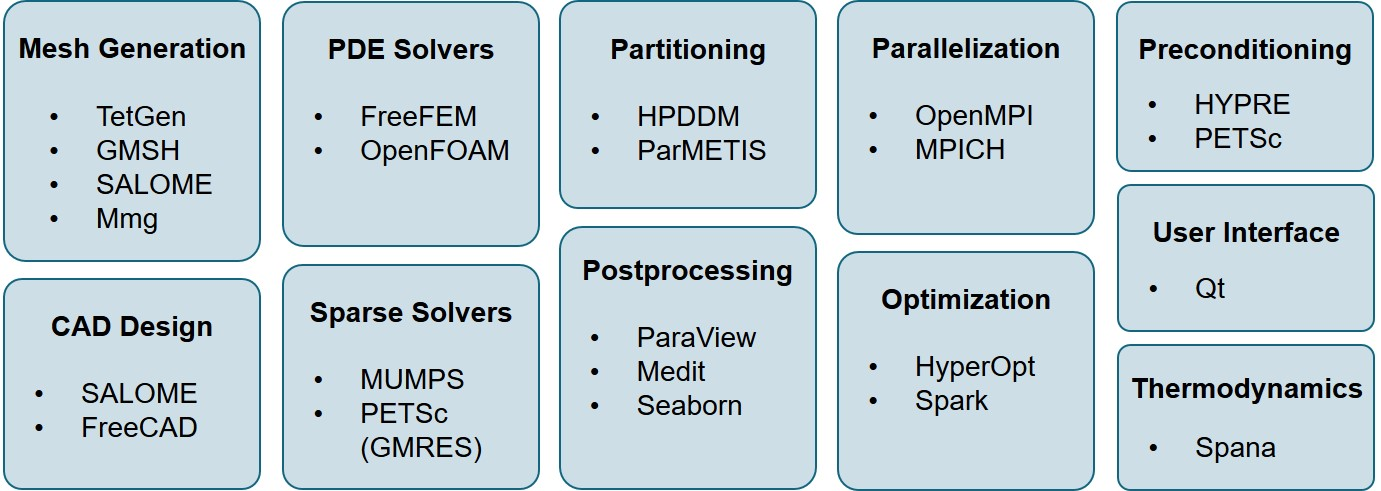
\includegraphics[width=\textwidth]{tools.jpg}
\caption[Overview of open-source tools and libraries used in this PhD]{An overview of tools and libraries used in this research, which are all free and open-source.} \label{fig:conclusion_tools}
\end{figure}



%As a summary, we should emphasize that this PhD was not possible without the freedom and control available in open-source scientific computing world. 



\subsection{Moving interface problems}

% defining BCs on an implicit interface

\subsection{High-performance computing and scaling}

%Building with different MPI implementations
%Inter-node communication
%Running parallel FF
%Mesh generation (parallel, sequential)
%Converting surface mesh to volume
%Scaling issues
%Memory issues
%Node types
%Visualization, GPU nodes
%Partitioning (METIS, ParMETIS)
%Storage
%Solving NS equation

\subsection{Certainty in chemical experiments}

% capturing the chemistry in math
% lack of certainty in chemical experiments, leading to difficulty in modeling

\section{Future perspectives}



%%%%%%%%%%%%%%%%%%%%%%%%%%%%%%%%%%%%%%%%%%%%%%%%%%
% Keep the following \cleardoublepage at the end of this file, 
% otherwise \includeonly includes empty pages.
\cleardoublepage

% vim: tw=70 nocindent expandtab foldmethod=marker foldmarker={{{}{,}{}}}
